 \documentclass[10pt,a4paper]{article}
\usepackage{geometry}
 \geometry{
 a4paper,
 total={170mm,257mm},
 left=20mm,
 top=20mm,
 }


\usepackage[utf8]{inputenc}
\usepackage[spanish]{babel}
\usepackage{graphicx}
\usepackage{wrapfig}
\usepackage{amssymb, amsmath, siunitx}
\usepackage{tikz}
\usepackage{enumitem}
\usepackage{svg}
\usepackage{tcolorbox}
\usepackage{pdfpages}
\usepackage{mathtools}

\title{Ecuaciones Generales}
\author{Antonio Escámez Álvarez}
\date{Mayo 2021}


\setlength{\parindent}{0cm}

\begin{document}

\maketitle
\newpage
\tableofcontents
\newpage

\section{Conservación de la masa}
De esta fórmula podemos extraer velocidades o áreas.
\begin{center}
    \begin{tcolorbox}[colback=yellow!40!white, colframe=red!50!black,title=Conservación de la masa]
    $$
        \underbrace{\frac{d}{dt} \left[\int_{V_c(t)}^{} \rho \,dV \right] }_{\substack{\text{Variación temporal del} \\ \text{volumen de control} \\ \text{} \\ \text{Estacionario $\xrightarrow{}$ 0}}} + \underbrace{\int_{\sum_c(t)}^{} \rho \left[\left(\vec{v} - \vec{v_c}\right) \cdot \vec{n} \right] \, d\sigma}_{\substack{{\text {Flujo convectivo}} \\ {}}} = 0
    $$
    \end{tcolorbox}
\end{center}
Elementos que se desprecian:
\begin{itemize}
    \item Variación temporal del volumen de control \textbf{SIEMPRE SE DESPRECIA} ya que consideramos que estamos en régimen estacionario.
    \item Cuando hablamos de flujo convectivo tenemos que ver si el flujo atraviesa nuestro elemento o no, es decir en la entrada y salida siempre vamos a tener flujo convectivo, pero en las paredes y elementos como álabes no, ya que el fluido no atraviesa las paredes ni el álabe.
    \item El volumen de control del flujo convectivo $\vec{v_c}$ se desprecia ya que nuestro volumen de control es 0
    \item El producto escalar de $\vec{v} \cdot \vec{n}$ se anula en el caso de que la velocidad y la normal sean perpendiculares 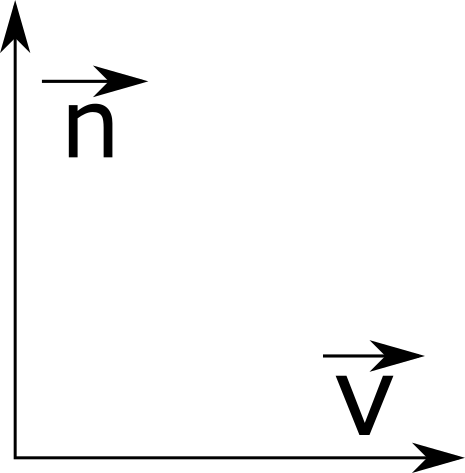
\includegraphics[scale = 0.2]{path833.png}
\end{itemize}

\section{Cantidad de movimiento}
De esta fórmula podemos extraer fuerzas principalmente.
\begin{center}
    \begin{tcolorbox}[colback=yellow!40!white, colframe=red!50!black,title=Cantidad de movimiento]
    $$
        \underbrace{\frac{d}{dt} \left[\int_{V_c(t)}^{} \rho \cdot \vec{v} \,dV \right] }_{\substack{\text{Variación temporal del} \\ \text{volumen de control} \\ \text{} \\ \text{Estacionario $\xrightarrow{}$ 0}}} + \underbrace{\int_{\sum_c(t)}^{} \rho \cdot \vec{v} \left[\left(\vec{v} - \vec{v_c}\right) \cdot \vec{n} \right] \, d\sigma}_{\substack{{\text {Flujo }} \\ {\text{Convectivo}}}} =
        \underbrace{\underbrace{-\int_{\sum_c(t)}^{}p \cdot \vec{n} \, d\sigma}_{\substack{\text{Término de } \\  {\text{Presiones}}}} + \underbrace{\int_{\sum_c(t)}^{}\vec{\vec{\tau}} \cdot \vec{n} \, d\sigma}_{\substack{\text{Esfuerzos } \\  {\text{Viscosos}}}}}_{\text{Fuerzas de superficie}} + \underbrace{\int_{V_c(t)}^{}\rho \cdot \vec{f_m} \, dV}_{\substack{\text{Fuerzas } \\  {\text{Masicas}}}}
    $$
    \end{tcolorbox}
\end{center}
\begin{itemize}
        \item El término de presiones se trabaja en manométricas $p = P - P_a$ y se puede eliminar cuando la presión sea atmosférica $P_a - P_a = 0$ o cuando la presión actué por igual en todo el elemento (que sea simétrico en todos los ejes)
        
        \item El término de esfuerzos viscosos hay que verlo como una fuerza de rozamiento, tenemos esfuerzos viscosos en las paredes y no tenemos en la entrada y salida.
        \begin{center}
            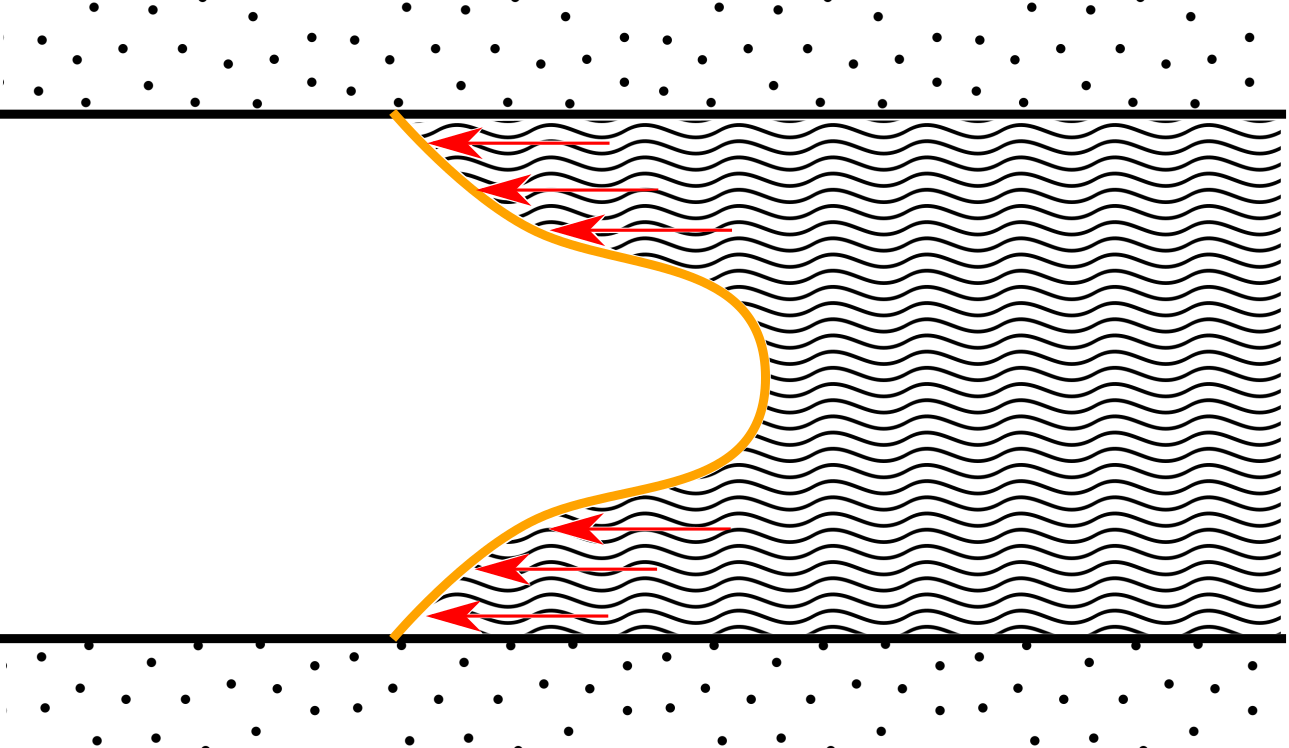
\includegraphics[scale = 0.4]{path1339.png}
        \end{center}
        
        \item Las fuerzas másicas son la de la gravedad y si el elemento gira aparece una fuerza centrifuga.
        
        \item Normalmente suele quedar un término de presión junto con el del esfuerzo viscoso que es a los que llamamos $-\vec{F}$. y que despejando obtenemos la fuerza que nos suelen pedir.
        
        
    \end{itemize}
    
\section{Momento cinético}
\begin{center}
    \begin{tcolorbox}[colback=yellow!40!white, colframe=red!50!black,title=Momento Cinético]
\begin{equation*}
\begin{split}
 \underbrace{\frac{d}{d_{t}}\left[\int_{V_{c(t)}} \rho \cdot\left(\vec{x}-\vec{x}_{0}\right) \wedge \vec{v} \, d V\right]}_{\substack{\text{Variación temporal del} \\ \text{volumen de control} \\ \text{} \\ \text{Estacionario $\xrightarrow{}$ 0}}} + \underbrace{\int_{\Sigma c(t)} \rho\left[\left(\vec{x}-\vec{x}_{0}\right) \wedge \vec{v}\right] \cdot\left[\left(\vec{v}-\vec{v}_{c}\right) \cdot \vec{n}\right] d \sigma}_{\substack{{\text {Flujo }} \\ {\text{Convectivo}}}} = \\
        \underbrace{\underbrace{-\int_{\Sigma(t)}\left(\vec{x}-\vec{x}_{0}\right) \wedge p \vec{n} \, d \sigma}_{\substack{\text{Término de } \\  {\text{Presiones}}}} + \underbrace{\int_{\Sigma c(t)}\left(\vec{x}-\vec{x}_{0}\right) \wedge(\vec{\vec{\tau}} \cdot \vec{n}) \, d \sigma}_{\substack{\text{Esfuerzos } \\  {\text{Viscosos}}}}}_{\text{Fuerzas de superficie}} + \underbrace{\int_{V_c(t)} \rho\left(\vec{x}-\vec{x}{0}\right) \wedge \vec{f}_{m} \, d V}_{\substack{\text{Fuerzas } \\  {\text{Masicas}}}}
\end{split}
\end{equation*}
    \end{tcolorbox}
\end{center}

\section{Ecuación de la energía}
\begin{center}
    \begin{tcolorbox}[colback=yellow!40!white, colframe=red!50!black,title=Ecuación de la energía]
\begin{equation*}
\begin{split}
\underbrace{\frac{d}{dt}\left[\int_{V_c(t)} \rho \cdot\left(e+\frac{v^{2}}{2}+g z\right) d V\right]}_{\substack{\text{Variación temporal del} \\ \text{volumen de control} \\ \text{} \\ \text{Estacionario $\xrightarrow{}$ 0}}}+\underbrace{\int_{\Sigma c(t)} \rho \cdot\left(e+\frac{v^{2}}{2}+g z\right) \cdot\left[\left(\vec{v}-\vec{v}_{c}\right) \cdot \vec{n}\right] d \sigma}_{\substack{{\text {Flujo }} \\ {\text{Convectivo}}}}= \\ \underbrace{-\int_{\Sigma c(t)} p \vec{v} \cdot \vec{n} d \sigma}_{\substack{\text{Término de } \\  {\text{Presiones}}}} +\underbrace{\int_{\Sigma c(t)} \vec{v} \cdot(\vec{\tau} \cdot \vec{n}) d \sigma}_{\substack{\text{Esfuerzos } \\  {\text{Viscosos}}}}+\underbrace{\int_{\Sigma c(t)} k(\nabla T \cdot \vec{n}) d \sigma}_{\substack{\text{Calor por } \\  {\text{Conducción}}}}+\underbrace{\int_{V_c(t)}\left(\dot{q}_{R}+\dot{q}_{Q}\right) d V}_{\substack{\text{Calor por } \\  {\text{radiación y reacción química}}}} + \underbrace{\int_{V_c(t)}^{}\rho \cdot \vec{f_m} \, dV}_{\substack{\text{Fuerzas} \\  {\text{Másicas}}}}
\end{split}
\end{equation*}
    \end{tcolorbox}
\end{center}

\end{document}
